\subsection{Polimerizzazione per quadruplo legame ad idrogeno}
\begin{frame}\frametitle{Polimerizzazione per quadruplo legame ad idrogeno}
\begin{columns}
 \column{0.5\linewidth}
Le unità in figura sono autocomplementari ed hanno altissima costante d'associazione. Il materiale in figura in basso ad \textbf{alta temperatura} si comporta come \textbf{fluido} con i monomeri separati, a \textbf{temperatura ambiente} è un \textbf{polimero ad alto peso molecolare}. 
\column{0.5\linewidth}
\begin{figure}{\centering{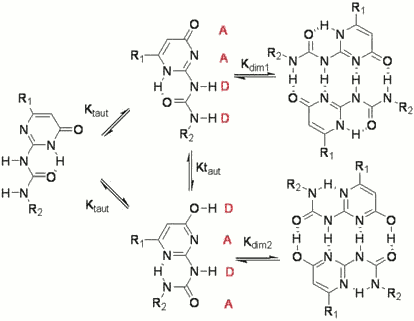
\includegraphics[width=1\textwidth]{legame_h/quadruplo-tautomeri.png}}}\end{figure}
\end{columns}\vspace{-5pt}
\begin{figure}{\centering{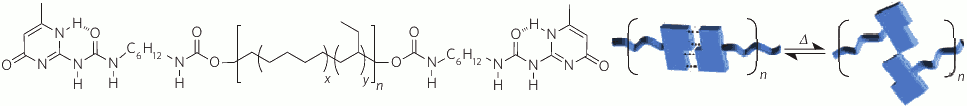
\includegraphics[width=1\textwidth]{legame_h/quadruplo.png}}}\end{figure}\vspace{-20pt}
\footnote{\tiny \leading{5pt} \fullcite{quadruplo} \\ \fullcite{quadruplo-polim}}
\end{frame}

\subsection{Reticolazione per legami ad idrogeno}
\begin{frame}\frametitle{Reticolazione per legami ad idrogeno}

La \textbf{varietà} strutturale \textbf{evita la cristallizzazione} nella \textbf{gomma}.
\begin{columns}
 \column{0.45\linewidth}
I nuclei poliacidi sono dimeri e trimeri di \textbf{acidi grassi} di origine vegetale. Viene plastificato con dodecano. Una volta \textbf{tagliato}, le superfici vanno \textbf{poste in contatto entro breve tempo} per \textbf{evitare} che le coppie spezzate \textbf{si riorganizzino} all'interno delle due superfici. Ha bassa deformabilità.

\column{0.6\linewidth}
\begin{figure}{\centering{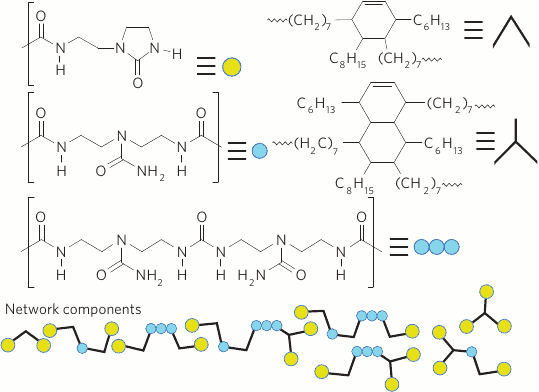
\includegraphics[width=1\textwidth]{legame_h/leibler.png}}}\end{figure}
\end{columns}
\footnote{\tiny \leading{5pt} \fullcite{leibler-nature}\\\fullcite{leibler-sintesi}\\\fullcite{leibler-2010}}
\end{frame}




\subsection{Reticolazione per $\pi-\pi$ stacking}
\begin{frame}\frametitle{Piccole molecole reticolate per  $\pi-\pi$ \emph{stacking}}

Per avere una interazione di \emph{stacking} abbastanza forte è stato usato un \textbf{aromatico elettronricco ed uno elettronpovero} insieme a legami ad idrogeno.

Il materiale presenta una intensa \textbf{colorazione rossa} a causa del trasferimento di carica. 

La \textbf{riparazione} avviene \textbf{perfettamente} ma solo a temperature maggiori di 50$^\circ$C.

\begin{figure}{\centering{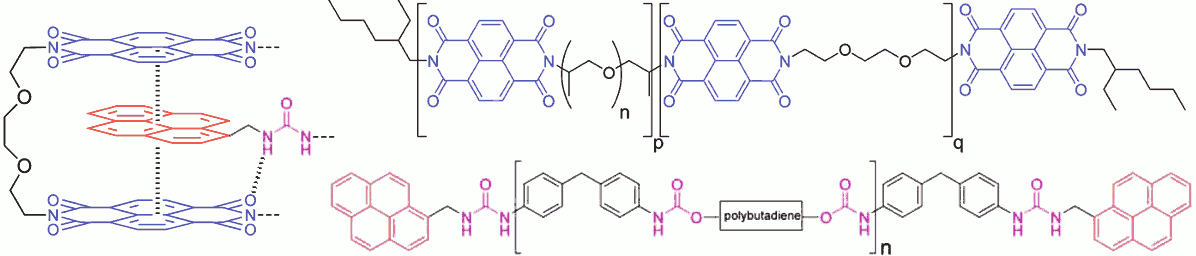
\includegraphics[width=0.9\textwidth]{legame_h/stacking.png}}}\end{figure}\vspace{-10pt}
\footnote{\tiny \leading{5pt} \fullcite{stacking}}
\end{frame}




\subsection{Reticolazione per interazione ionica}
\begin{frame}\frametitle{Reticolazione per interazione ionica}
Gli \textbf{ionomeri} sono \textbf{poli acidi carbossilici neutralizzati} con fino al 15\% eq di \ce{NaOH} aventi \textbf{interazioni} fisiche tra le \textbf{catene laterali ioniche}. 


Quando si ha l'impatto di un \textbf{proiettile} questo porta a \textbf{fusione} il materiale e forma un foro. Dunque il fuso \textbf{chiude elasticamente} il foro, successivamente per \textbf{interdiffusione} avviene la saldatura.  

\footnote{\tiny \leading{5pt} \fullcite{ionomeri}}
\begin{columns}
 \column{0.5\linewidth}
\begin{figure}{\centering{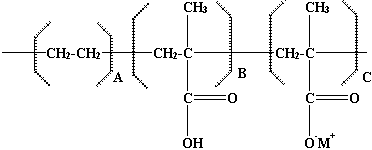
\includegraphics[width=0.9\textwidth]{legame_h/surlyn.png}}}\end{figure}
\column{0.5\linewidth}
\begin{figure}{\centering{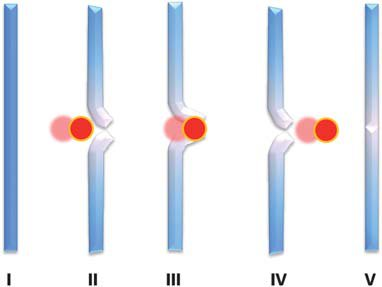
\includegraphics[width=0.6\textwidth]{legame_h/ionomero.jpg}}}\end{figure}
\end{columns}
\end{frame}




\subsection{Altro}
\begin{frame}\frametitle{Altro}
Molti altri sistemi non sono stati trattati, ad esempio:\vspace{-10pt}
\begin{columns}
 \column{0.6\linewidth}
\begin{figure}{\centering{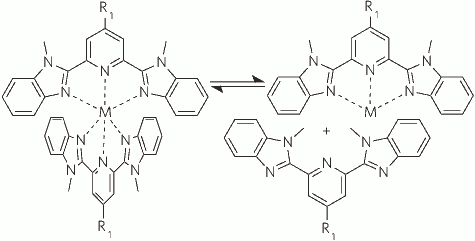
\includegraphics[width=0.8\textwidth]{legame_h/altri-metallo.png}}}\end{figure}
\column{0.4\linewidth}
\begin{figure}{\centering{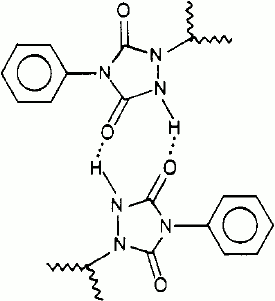
\includegraphics[width=0.4\textwidth]{legame_h/altri-2h.png}}}\end{figure}
\end{columns}
\begin{figure}{\centering{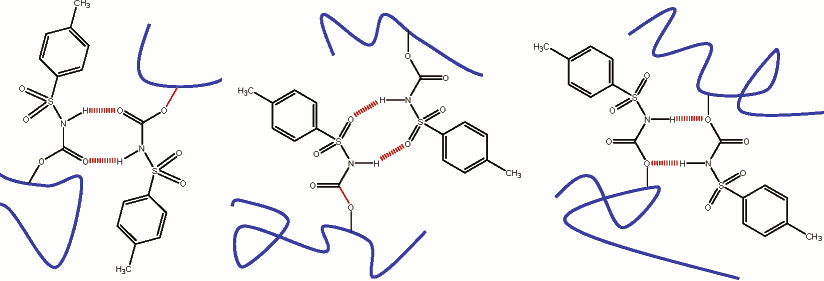
\includegraphics[width=0.9\textwidth]{legame_h/altri-solfo.png}}}\end{figure}

\end{frame}
